
\documentclass[../D+Manual.tex]{subfiles}
\begin{document}

\chapter{Remote Calculations}
\label{chp:remoteCalculations}

\begin{quote}
	Magnetism is one of the Six Fundamental Forces of the Universe, with the other five being Gravity, Duct Tape, Whining, Remote Control, and The Force That Pulls Dogs Toward The Groins Of Strangers.\\
	\hspace*{\fill} \textit{Dave Barry}	
\end{quote}

In the \texttt{Start Menu}, under \texttt{D+}, there is a \texttt{Remote D+} option. If you do not find this option, go to \path{C:\ProgramData\Microsoft\Windows\Start Menu\Programs\D+}, and run \texttt{Remote D+} from there. 

The main difference between \texttt{Remote D+} and the local version of D+ is where the computations take place.
In the local version, a local copy of the backend is run, using your computers resources.
In the remote version, computations are carried out on a server running the backend with the communications handled over the internet.

\begin{wrapfigure}{r}{0.4\textwidth}
	\vspace{-20pt}
	\centering
	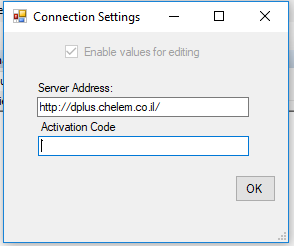
\includegraphics[width=0.95\linewidth]{ConnectionSettings}
\end{wrapfigure}
In the directory with \path{DPlus.exe} (or \path)
there may be an additional file named \path{Server.dserv}.
This is a plain text file with the servers URL and an optional port number.
If this file does not exist, then a window will open when starting D+ that looks like the one to the right, just without the Server Address.
In the \texttt{Server Address} field, enter the servers URL (and port number if it is different than 80).

When subsequently starting D+, it will attempt to connect to the same server.
In order to change the server, either delete the \path{Server.dserv} file before launching, or choose \texttt{Configure Server} under the \texttt{Settings} menu.

You will then need an activation code like this: 
\texttt{fd8d997a007d96a320d556846a48d340315faf2e}. 
If you do not have a GPU on your computer, running long calculations will be faster on a server with GPU.


 
\end{document}